\documentclass{standalone}
\usepackage{tikz}
\usepackage{ctex,siunitx}
\usepackage{tkz-euclide}
\usepackage{amsmath}
\usetikzlibrary{patterns, calc}
\usetikzlibrary {decorations.pathmorphing, decorations.pathreplacing, decorations.shapes,}
\begin{document}
\small
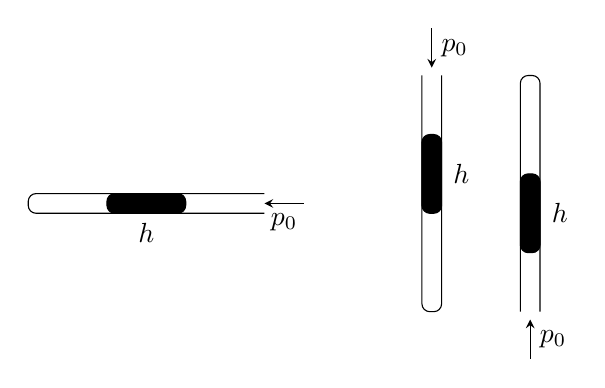
\begin{tikzpicture}[>=stealth,scale=1.0]
  \draw[rounded corners=0.1cm](-2,0)--(-5,0)--(-5,-.25)--(-2,-.25);	
  \draw[rounded  corners=0.1cm, fill=black](-4,-.25) rectangle (-3,0);		
  \node at (-3.5,-.5){$h$};
  \draw[<-](-2,-0.125)--node[below]{$p_0$}(-1.5,-.125);
  \draw[rounded corners=0.1cm](0,1.5)--(0,-1.5)--(.25,-1.5)--(.25,1.5);
  \draw[rounded  corners=0.1cm, fill=black](0,-.25) rectangle (.25,.75);
  \node at (.5,.25){$h$};
  \draw[<-](0.125,1.6)--node[right]{$p_0$}(0.125,2.1);
  \draw[rounded corners=0.1cm](1.25,-1.5)--(1.25,1.5)--(1+.5,1.5)--(1+.5,-1.5);
  \draw[rounded  corners=0.1cm, fill=black](1.25,-0.75) rectangle (1+.5,.75-0.5);
  \node at (1.75,-0.25){$h$};
  \draw[<-](1.375,-1.6)--node[right]{$p_0$}(1.375,-2.1);
\end{tikzpicture}
\end{document}